%!xelatex = 'xelatex --halt-on-error %O %S'

\documentclass{thuemp}
\begin{document}

% 标题,作者
\emptitle{光栅衍射实验报告}
\empauthor{江灿}{2019011325}

% 奇数页页眉 % 请在这里写出第一作者以及论文题目
\fancyhead[CO]{{\footnotesize 江灿: 光栅衍射实验报告}}


%%%%%%%%%%%%%%%%%%%%%%%%%%%%%%%%%%%%%%%%%%%%%%%%%%%%%%%%%%%%%%%%
% 关键词 摘要 首页脚注
%%%%%%%%关键词
\Keyword{霍尔效应,副效应,磁阻测量}
\twocolumn[
\begin{@twocolumnfalse}
\maketitle

%%%%%%%%摘要
\begin{empAbstract}
霍尔效应是电磁效应的一种,这一现象是美国物理学家霍尔(E.H.Hall,1855—1938)于1879年在研究金属的导电机制时发现的。 当电流垂直于外磁场通过半导体时,载流子发生偏转,垂直于电流和磁场的方向会产生一附加电场,从而在半导体的两端产生电势差,这一现象就是霍尔效应,这个电势差也被称为霍尔电势差。
霍尔效应在应用技术中特别重要。根据霍尔效应做成的霍尔器件,就是以磁场为工作媒体,将物体的运动参量转变为数字电压的形式输出,使之具备传感和开关的功能。

\end{empAbstract}
\empfirstfoot{2022-04-03}{软件02}{双日下M}{7号}
%%%%%%%%首页角注,依次为实验时间、报告时间、学号、email
\end{@twocolumnfalse}
]
%%%%%%%%!首页角注可能与正文重叠,请通过调整正文中第一页的\enlargethispage{-3.3cm}位置手动校准正文底部位置:
%%%%%%%%%%%%%%%%%%%%%%%%%%%%%%%%%%%%%%%%%%%%%%%%%%%%%%%%%%%%%%%%
%  正文由此开始
\wuhao 
%  分栏开始

\section{实~~验~~目~~的}
略

%%%%%%%%%%%%%%%%%%%%%%%%%%%%%%%%%%%%%%%%%%%%%%%%%%%%%%%%%%%%%%%%
\section{实~~验~~仪~~器}
略
\section{实~~验~~原~~理}
略
%%%
\section{实~~验~~步~~骤} 
略
%%%%%%%%%%%%%%%%%%%%%%%%%%%%%%%%%%%%%%%%%%%%%%%%%%%%%%%%%%%%%%%%
%%%%%%%%%%%%%%%%%%%%%%%%%%%%%%%%%%%%%%%%%%%%%%%%%%%%%%%%%%%%%%%%
\newpage
\section{实~~验~~数~~据}

\subsection{$U_{H}$与I关系及$K_{H},R_{H},n$的计算}

由实验室提供的表格查得$I_{M}$=500mA时,$B_{0}$=123.7mT
由实验所测得数据制作的$U_{H}-I$关系曲线如图
\begin{figure}[H]
	\centering
	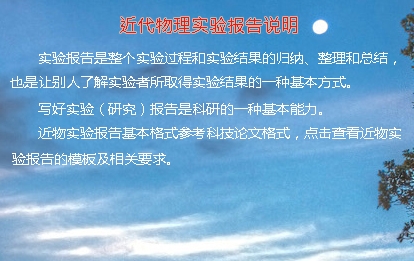
\includegraphics[width=0.8\linewidth]{./image/example.jpg}
	\caption{$U_{H}$=I} \label{fig:eg}
\end{figure}
可见,$U_{H}$,I成线性关系.

直线斜率k=23.30714275,相关系数r=0.9999901842

由$U_{H}=R_{H}\frac{IB}{d}=K_{H}IB$,故$k=\frac{R_{H}B}{d}=K_{H}$,所以有
\[R_{H}=\frac{kd}{B}=\frac{23.30714275x3x10^{-6}}{123.7x10^{-3}}\approx5.65239x10^{-4} \Omega·m/T\]
\[K_{H}=\frac{k}{B}=188.4156 \Omega/T\]
\[\delta k =S_{K}=k\sqrt{\frac{\frac{1}{r^{2}-1}}{n-2}}\approx0.04607\Omega\]
\[\delta R_{H} = \frac{d}{B}\delta k \approx 1.1x10^{-6} \Omega·m/T\]
\[\delta K_{H} = \frac{1}{B}\delta K \approx 0.4\Omega/T\]
故\[R_{H}=(5.653\pm0.011)x10^{-4} \Omega ·m/T\]
\[K_{H}=(188.4\pm 0.4 )\Omega /T\]
又$R_{H}=\frac{1}{ne}$,故\[n=\frac{1}{R_{H}e}=1.1031X10^{22}m^{-3}\]
\[\delta n =\frac{\delta R_{H}}{R_{H}^{2}e}\approx2.1x10^{19}m^{-3}\]
故\[n=(1.1031\pm0.0021)X10^{22}m^{-3}\]
不等位效应$U_{0}$的确定:
由实验原理$U=f(U_{H},U_{E},U_{N},U_{R},U_{O},U_{S})$,f表示求和,式中$U_{E}$很小可略去,故
$U=f(U_{H},U_{E},U_{N},U_{R},U_{O},U_{S})=U_{H}+U_{N}+U_{R}+U_{P}+U_{S}$

不妨设+B,+I的条件下参与求和的各电压均取正值

由于$U_{H}$正负与I,B方向有关,$U_{N},U_{R}$正负只与B方向有关,$U_{O}$方向只与I方向有关,$U_{S}$与I,B无关,故
\[U_{1}(+B,+I_{H})=f(U_{H},U_{N},U_{R},U_{O},U_{S})\]
\[U_{2}(+B,+I_{H})=f(-U_{H},U_{N},U_{R},-U_{O},U_{S})\]
\[U_{3}(+B,+I_{H})=f(U_{H},-U_{N},-U_{R},-U_{O},U_{S})\]
\[U_{4}(+B,+I_{H})=f(-U_{H},-U_{N},-U_{R},U_{O},U_{S})\]
所以
\[\frac{1}{4}(U_{1}+U_{3}-U_{2}-U_{4}=U_{H}\]
\[\frac{1}{4}[(U_{1}-U_{2})-(U_{3}-U_{4})]=U_{O}\]
故\[U_{O}=\frac{1}{4}(U_{1}-U_{2}-U_{3}+U-{4})\]
现将实验1中各结果整理如下
\[R_{H}=(5.653\pm0.011)x10^{-4} \Omega ·m/T,K_{H}=(188.4\pm 0.4 )\Omega /T\]
\[n=(1.1031\pm0.0021)X10^{22}m^{-3},U_{O}=\frac{1}{4}(U_{1}-U_{2}-U_{3}+U-{4})\]
\subsection{标定$I_{M}$与B的关系}
有实验数据可得
\[B=\frac{U_{H}}{K_{H}I},I=4.00mA,K_{H}=188.4 \Omega/T\]
由此可作出B-$I_{M}$曲线,
\begin{figure}[H]
	\centering
	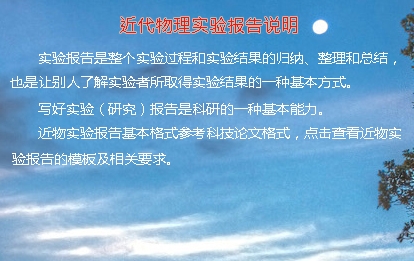
\includegraphics[width=0.8\linewidth]{./image/example.jpg}
	\caption{B-$I_{M}$} \label{fig:eg}
\end{figure}
由曲线可以看出B与$I_{M}$成线性(基本为正比)关系,这与理论相符.用计算器可求得拟合直线的方程:
\[B=0.4065+0.2472I_{M}\]
$I_{M}$的单位为mA,B单位为mT.
相关系数r=0.99999243
\subsection{锑化铟磁阻器件的磁电阻效应}
由实验数据整理得
\[R(B)=\frac{U_{CD}}{I} ,I=1.50mA,\]
\[\delta R=R(B)-R(O),B=0.4065+2472I_{M}(mT)\]
由此可绘出$\delta R/R(O)~B$的关系曲线
\begin{figure}[H]
	\centering
	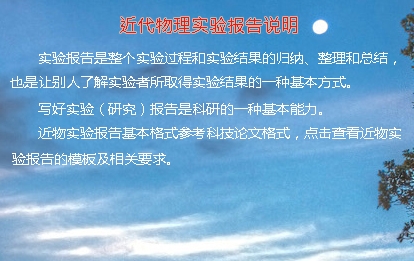
\includegraphics[width=0.8\linewidth]{./image/example.jpg}
	\caption{$\delta R/R(O)~B$} \label{fig:eg}
\end{figure}
由曲线走势进行如下回归分析:

取前六点进行二次回归,有
\[\delta R/R(O)=0.0803B^{2}+1.2452B-5.0797,r^{2}=0.9991\]
相关程度高

取后六点进行线性回归,有
\[\delta R/R(O)=2.9426B+414.32,r^{2}=0.9989\]
相关程度较高

于是在磁场较弱时,$ \delta R/R(O) $与B有着二次函数的关系,曲线为抛物线.
磁场较强时,$ \delta R/R(O) $存在线性关系,曲线为直线.

抛物线与直线间光滑过渡.
与原理中部分内容符合较好
\subsection{磁极间隙水平方向磁场的分布曲线}
由实验数据整理得:

\[B=\frac{U_{H}}{K_{H}I},I=4.00mA,K_{H}=1.884 \Omega/T\]
	实验时的励磁电流$I_{M}=500mA$
由此可作出实验曲线
\begin{figure}[H]
	\centering
	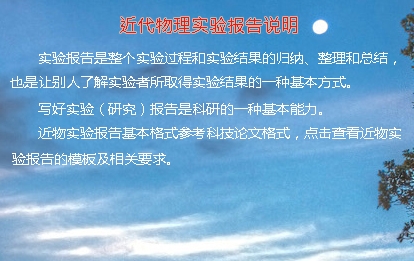
\includegraphics[width=0.8\linewidth]{./image/example.jpg}
	\caption{B~X} \label{fig:eg}
\end{figure}
曲线有对称性,对称轴大致在气隙中心位置.从曲线中可以看出,随着x的增大,B先是逐渐增大到某个值,在一定范围内保持恒定,然后又逐渐减小.增加的速度先慢后快,后由快变慢.下降的速度亦然.

从曲线中可以看出,电磁铁气隙中心的磁场为均匀磁场,且磁感应强度最大.
\subsection{判断载流子类型}
\begin{figure}[H]
	\centering
	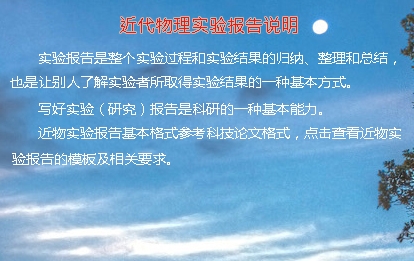
\includegraphics[width=0.8\linewidth]{./image/example.jpg}
	\caption{载流子} \label{fig:eg}
\end{figure}
电流方向如图中标示.由左手定则,不管载流子是电子和空穴,均会发生向下的偏转.有由于3端的电势低,故发生偏转的是电子.也即载流子为电子
\subsection{霍尔片中载流子的迁移率μ}
\[\mu=\frac{v}{E}=\frac{v}{J/\sigma}=\sigma\frac{v}{nevbd/(bd)}=\frac{\sigma}{ne}=\sigma R_{H}\]
故欲测μ即是要测霍尔片的电导率$\sigma$

又因为电阻R=$ \frac{U_{cd}}{I}=\frac{1}{\sigma}\frac{L}{bd} $

故
\[\sigma = \frac{L}{bd}\frac{I}{U_{cd}},I=\frac{\sigma bd}{l}U_{cd}\]
可见由$I-U_{cd}$的曲线的斜率可求出$\sigma$
\begin{figure}[H]
	\centering
	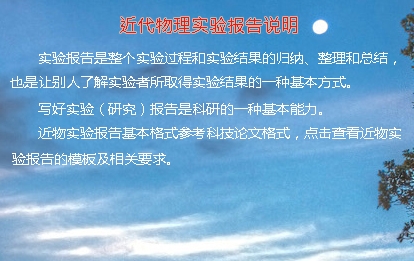
\includegraphics[width=0.8\linewidth]{./image/example.jpg}
	\caption{载流子} \label{fig:eg}
\end{figure}
所做图像如图,回归直线方程:I=-0.1041+1.0935$U_{cd}$
r=0.99965
故斜率k=1.0935mA/V
\[\delta k \approx S_{K}=k\sqrt{\frac{1/r^{2}-1}{n-2}}\approx0.010935mA/V\]
\[k=\frac{\sigma bd}{l}\]
\[\sigma=\frac{k l}{b d}\approx1093.5S/m\]
\[\delta \sigma =\frac{l}{bd}\delta k\approx11s/m\]
\[\sigma=(1094\pm11)S/m\]
\[\mu=\sigma R_{H}=0.618438T^{-1}\]
\[ln\mu=ln\sigma+lnR_{H}\]
\[\frac{\partial ln \mu}{\partial \sigma}=\frac{1}{\sigma},\frac{\partial lu \mu}{\partial R_{H}}=\frac{1}{R_{H}}\]
\[\frac{\delta \mu}{\mu}=\sqrt{(\frac{\delta \sigma}{\sigma})^{2}+(\frac{\delta_{RH}}{R_{H}})^{2}}
=1.0241x10^{-2}\]
\[\delta \mu =\mu \frac{\delta \mu}{\mu}\approx6x10^{-3}T^{-1}\]
\[\mu=(0.618\pm0.006)T^{-1}\]


\subsection{往届学生报告中常见问题与不足}
正文内容正文文字五号宋体正文内容正文文字五号宋体正文内容正文文字五号宋体正文内容正文文字五号宋体正文内容正文文字五号宋体正文内容正文文字五号宋体正文内容。
\subsubsection{三级标题}
\subsubsection{只给数据和结果,没有对结果所反映的物理规律做理论分析及数据误差分析;}
\subsubsection{数据及结果直接给出,没有必要的实验条件说明和所用物理计算公式;}
\subsubsection{结果以图、表给出时,图、表不规范(缺少坐标分度、物理量及其单位等);}
正文内容正文文字五号宋体正文内容正文文字五号宋体正文内容正文文字五号宋体正文内容正文文字五号宋体正文内容正文文字五号宋体正文内容正文文字五号宋体正文内容。
\subsection{报告中公式、字母的规范写法}
公式全文统一编号,如公式为
\begin{equation}\label{EQ1}
\frac{\partial u}{\partial x}+\frac{\partial v}{\partial y}+\frac{\partial w}{\partial z}=0
\end{equation}
式中,$u$是××××(单位);$v$是×××(单位);$w$是××(单位)。

对于公式,应全文统一连续编号,如式\eqref{EQ1}……一般情况下,需要引用的或重要的公式才编号。在文中引用时,用“式(编号)”表示。
后文不再提及的,可以不编号。如
\begin{equation*}
1 + 1 + 3 = 5
\end{equation*}

对于公式中首次出现的量的符号,按照其在式中出现的顺序,用准确、简洁的语句对其进行逐一解释。公式中变量应尽量避免复合上下角标的使用;尽量少用3层关系的上下标,同时应尽量减少不必要的公式推导。

\subsection{报告中图的规范要求}
插图全文顺序编号。插图内容应与正文内容密切结合,每幅图前都应有相应的引出或介绍文字。图形应保证线条清晰,图形大小应适应版面要求,合理布局,图内如有标注或说明性文字时应清晰可辨。图中除了物理量符号及单位外一律用中文,同一图中的不同曲线应用不同线型表示。插图分辨率要大于600PPI。

正文文字中先见文,后见图,图号全文统一按顺序编号,如图\ref{fig:eg}所示。图中文字为6号,图线必须清晰可辨坐标轴的物理量和单位不可缺。




\subsection{报告中表的规范}
推荐使用标准“三线表”(如表\ref{tab:eg1}所示。),内容易混淆时可加辅助线进行辅助说明。按表格在文中出现的顺序,用阿拉伯数字对其进行编号,全文顺序编号。应有相应的表题且每个表格前都应有相应的引出或介绍文字。

图、表应在文中有相应表述,即图、表的号应在文中引出,以先见文后见图、表为原则。每个图、表都必须有图名、表名,并且有编号。图号、表号应全文统一连续排列,即,应按照图1、图2……排列不应按小结编号。图片中的文字、线条应当清晰可辨,图片像素(DPI)在300以上。
表格推荐采用全线表,表头中使用量符号/量单位形式。如表\ref{tab:eg2}所示。

\begin{table}[h]
\centering
\captionnamefont{\wuhao\bf\heiti}
\captiontitlefont{\wuhao\bf\heiti}
\caption{三线表示例} \label{tab:eg1}
\liuhao
\begin{tabular}{cccc}
\toprule
{编号} &  {直径}/\si{\metre} & {静温}/\si{\kelvin} & {时间}/min\\
\midrule 
4 & 0.0349 & 268.15 & 30\\
5 & 0.01905 & 268.15 & 30\\
\bottomrule
\end{tabular}
\end{table}

\begin{table}[h]
\centering
\captionnamefont{\wuhao\bf\heiti}
\captiontitlefont{\wuhao\bf\heiti}
\caption{全线表示例} \label{tab:eg2}
\liuhao
\begin{tabular}{|c|c|c|c|c|}
\hline
U/V & I/mA & v/km·h$^{-1}$ & x/mm & p/MPa \\ \hline
\textit{12} & \textit{30} & \textit{80} & \textit{55} & \textit{110} \\ \hline
\textit{24} & \textit{34} & \textit{90} & \textit{60} & \textit{111} \\ \hline
\end{tabular}
\end{table}

\subsection{报告中英文缩略语的规范}
文中的英文缩略语应在首次出现时给出中文含义以及英文全称后再使用。例如,全球定位系统(Global Positioning System,GPS)。


\subsection{外文字母}
\subsubsection{斜体外文字母用于表示量的符号,主要用于下列场合}

\begin{enumerate}
\renewcommand{\labelenumi}{(\theenumi)}
\item 变量符号、变动附标及函数。
\item 用字母表示的数及代表点、线、面、体和图形的字母。
\item 特征数符号,如Re (雷诺数)、Fo (傅里叶数)、Al (阿尔芬数)等。
\item 在特定场合中视为常数的参数。
\end{enumerate} 

\subsubsection{正体外文字母用于表示名称及与其有关的代号,主要用于下列场合}
\begin{enumerate}
\renewcommand{\labelenumi}{(\theenumi)}
\item 有定义的已知函数(例如$\sin$, $\exp$, $\ln$等)。
\item 其值不变的数学常数(例如$\mathrm{e} = 2.718 281 8\cdots)$及已定义的算子。
\item 法定计量单位、词头和量纲符号。
\item 数学符号。
\item 化学元素符号。
\item 机具、仪器、设备和产品等的型号、代号及材料牌号。
\item 硬度符号。
\item 不表示量的外文缩写字。
\item 表示序号的拉丁字母。
\item 量符号中为区别其他量而加的具有特定含义的非量符号下角标。
\end{enumerate} 
%%%%%%%%%%%%%%%%%%%%%%%%%%%%%%%%%%%%%%%%%%%%%%%%%%%%%%%%%%%%%%%%
\begin{figure}[H]
	\centering
	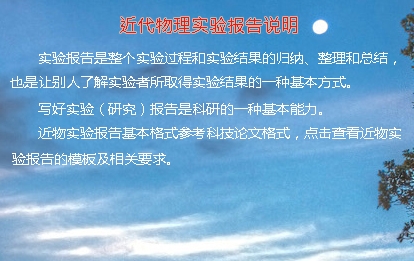
\includegraphics[width=0.8\linewidth]{./image/example.jpg}
	\caption{图片示例} \label{fig:eg}
\end{figure}

\section{思~~考~~题}

\subsection{如何计算实验中霍尔片载流子迁移率}
由"实验数据处理",$\mu=\Omega R_{H}$,其中$\Omega$为霍尔片的电导率,$R_{H}$为霍尔系数.具体计算过程将数据处理部分.
\subsection{如何观察不等位效应?如何消除不等位效应对测量带来的影响?}
将电磁铁的激励电流切断,B=0,此时霍尔片两侧面间仍有电位差.
改变电流$I_{H}$的方向,此电位差正负改变,这就是观察不等位效应的方法.
测量出$(+B,+I_{H}),(+B,-I_{H}),(-B,I_{H}),(-B,+I_{H})$下的电势差$U_{1},U_{2},U_{3},U_{4}$,并按式$U_{H}=\frac{1}{4}U_{1}-U_{2}+U_{3}-U_{4}$计算即可消除不等位效应,理由在数据处理部分已经给出.
\subsection{如何利用霍尔效应测量磁场?}
给霍尔片通以电流I,测出片上的霍尔电压$U_{H}$,即可通过式$ B=\frac{U_{H}}{K_{H}I} $计算出磁场,$K_{H}$课用实验的方法确定.
%%%%%%%%%%%%%%%%%%%%%%%%%%%%%%%%%%%%%%%%%%%%%%%%%%%%%%%%%%%%%%%%
\section{实~~验~~总~~结}
通过这次实验,我对于霍尔效应有了更加直观,深入的认识.学会了消除霍尔副效应的方法.本次实验内容丰富,各个小实验之间联系密切,前面实验的结构直接影响到了后面的实验.这让我对物理实验的方法有了更深刻的认识,对物理现象内在的联系有了进一步的体会.
%%%%%%%%%%%%%%%%%%%%%%%%%%%%%%%%%%%%%%%%%%%%%%%%%%%%%%%%%%%%%%%%
%  参考文献
%%%%%%%%%%%%%%%%%%%%%%%%%%%%%%%%%%%%%%%%%%%%%%%%%%%%%%%%%%%%%%%%
%  参考文献按GB/T 7714-2015《文后参考文献著录规则》的要求著录. 
%  参考文献在正文中的引用方法:\cite{bib文件条目的第一行}

\renewcommand\refname{\heiti\wuhao\centerline{参考文献}\global\def\refname{参考文献}}
\vskip 12pt

\let\OLDthebibliography\thebibliography
\renewcommand\thebibliography[1]{
  \OLDthebibliography{#1}
  \setlength{\parskip}{0pt}
  \setlength{\itemsep}{0pt plus 0.3ex}
}

{
\renewcommand{\baselinestretch}{0.9}
\liuhao
\bibliographystyle{gbt7714-numerical}
\bibliography{./TempExample}
}


\end{document}
